\documentclass[11pt]{article}
\usepackage[margin=1in]{geometry}
\usepackage{amsmath,amssymb,booktabs,graphicx,float}
\usepackage{pgfplots}\pgfplotsset{compat=1.18}
\usepackage{hyperref,xcolor}
\usepackage{algorithm,algpseudocode}
\title{\textbf{Aurelius Frontier Research Report:\\Measured Mechanisms for Efficient Frontier-Class LLMs\\
SISA $\cdot$ AEX-KV $\cdot$ MoK/LDK $\cdot$ Hybrid Architecture}}
\author{Christien Antonio \\ Aurelius Lab}
\date{August 5, 2026}

\newcommand{\sisa}{SISA}
\newcommand{\kl}{\mathrm{KL}}

\begin{document}
\maketitle

\begin{abstract}
We report a measurement-first research program toward frontier-class language
model efficiency. All claims are backed by executed probes on real model
weights (Qwen3-1.7B, Qwen2.5 family) and fast-cell training runs (nanochat
d6, 82M tokens). Contributions: (1) \sisa{}, a training-free, query-conditioned
sparse-attention indexer driven by the model's own binding circuit (heads
\{3,11\}), with a measured window law $W_{\mathrm{req}} \approx 1.1$--$1.3
\times$ horizon; (2) AEX-KV, a bit-exact lossless KV codec (1.135$\times$ on
real forward KV) that makes eviction \emph{reversible} ($\kl$ 1.70
$\rightarrow$ 0.00, measured); (3) a falsifier-first evaluation of recurrent
state (MoK) showing the gated-delta recurrence loses distance capacity to a
plain additive recurrence, and a new accumulate-only state design (LDK) that
outperforms both at long distance; (4) falsifications of clustered KV reads
(HCA 6.06 vs \sisa{} 1.70 $\kl$) and field-preserving clustering (FPC 7.09);
(5) a fully-specified hybrid architecture (KV=1, q-loRA, MoE, indexed
attention) with a running fast-cell gate. Every number in this report is
measured; every negative result is recorded.
\end{abstract}

\tableofcontents

\section{Introduction}
\label{sec:intro}
The Aurelius program targets frontier-class efficiency on constrained
hardware (Apple Silicon, GB10-class 128GB boxes, free-tier GPUs). Our thesis:
the read side of attention is where a frozen model's own signals are richest,
and losslessness is a first-class requirement. Section~\ref{sec:sisa} details
\sisa{}; Section~\ref{sec:aex} AEX-KV; Section~\ref{sec:mok} the MoK/LDK
state-memory investigation; Section~\ref{sec:fals} the clustering
falsifications; Section~\ref{sec:hybrid} the hybrid architecture; and
Section~\ref{sec:disc} positions the results against concurrent frontier
work (DeepSeek-V4 config-verified, StreamIndex, VarRate, AnchorKV, DART).

\section{Methods}
\label{sec:methods}
All CPU probes: Qwen3-1.7B (fp32, M1 Pro 32GB), transformers with
\texttt{attn\_implementation="eager"}, manual per-layer forward to capture
K/V and logits. Fast-cell training: nanochat fork, d6 (384-dim, 6 layers,
6 heads, 64 head-dim, seq 512, batch 16\,384, 5000 iters, 82M tokens,
Muon optimizer). Every training run logs val/bpb on a fixed holdout. All
comparisons are sequential fair runs (same 4--8 OMP threads).

\section{Self-Indexed Sparse Attention (SISA)}
\label{sec:sisa}
\sisa{} uses the model's own early-layer attention as a training-free
indexer: given a structured context (ledger records with key/value fields),
the binding circuit (heads \{3,11\} at the calibrated layer, window law
$W \ge W_{\mathrm{req}}$) scores candidate records by field mass, and the
budget $B$ evicts the lowest-mass tokens, compressing the rest into
$G$ residual groups (delta58 protocol).

\subsection{Binding circuit}
\begin{table}[H]\centering\small
\begin{tabular}{llrrr}
\toprule
Model & Layer & Head & id-frac & Note \\
\midrule
Qwen3-1.7B & 2 & 11 & 0.74--0.85 & dominant; head 3 secondary \\
Qwen3-1.7B & 2 & 3 & -- & selector (H4b: read-only) \\
Qwen2.5-1.5B & 5 & 11 & 0.92 & same absolute index \\
Qwen2.5-0.5B & 3 & \{0,5\} & -- & early quarter \\
Qwen2.5-7B-Inst & 2 & 4 & 0.14 & qualified \\
TinyLlama & -- & none & -- & family boundary (0/3) \\
\bottomrule
\end{tabular}
\caption{Head-role law: binding lives in the early quarter; absolute head
index scales with head count (calibrate per model).}
\end{table}

\subsection{Window law}
Measured with sliding-window masking (addition semantics, triu-correct):
\begin{equation}
W_{\mathrm{req}}(R) \approx (1.1\text{--}1.3) \cdot H(R),
\label{eq:windowlaw}
\end{equation}
where $H$ is the query-to-target horizon. Verified at $R \in \{15,30,60\}$
(Qwen3-1.7B: 300/251=1.20, 600/457=1.31, 1000/892=1.12) and replicated on
Qwen2.5-1.5B. Implication: any windowed architecture serving $\ge 2$K
contexts must keep the binding layer full-context.

\subsection{Leaderboard (measured)}
\begin{table}[H]\centering\small
\begin{tabular}{lccccc}
\toprule
Policy & Mean KL & vs U & Oracle-eq & Notes \\
\midrule
Uniform (U) & 6.26 & --- & no & strided drop \\
Random & 6.27 & +0.00 & no & 1/3 admission \\
Oracle Q & 2.83 & -3.43 & yes & privileged target span \\
\sisa{} (B=135) & 1.51 & -4.75 & 8/9 & attention-ranked drop \\
\bottomrule
\end{tabular}
\caption{6-qid battery: $t=-4.62$, $p=0.006$ vs U.}
\end{table}

\subsection{H2/H4/H4b/H6: indexer mechanics}
\begin{itemize}
\item H2: 2-head readout suffices (corr 0.944--0.990 vs full-head mass).
\item H4: under full context, zeroing heads \{3,11\} leaves p(digit)
$\approx 0.999$ (selector/reader split).
\item H4b: under eviction, zeroing head OUTPUT changes nothing
(ratio 0.998--1.000) --- the indexer is read-only; necessity lives in the
attention pattern itself.
\item H6: end-to-end with the 2-head indexer reproduces the oracle drop set
exactly (KL 2.0834/2.7934/3.1565 identical).
\end{itemize}

\section{AEX-KV: Bit-Exact Lossless KV Compression}
\label{sec:aex}
AEX-KV (21 reversible modes; zstd frames; per-block CRC32) satisfies
$\mathrm{decode}(\mathrm{encode}(X)) = X$ as uint16, preserving subnormals,
infinities and NaN payloads.

\subsection{Real-forward capacity (corrected)}
\begin{table}[H]\centering\small
\begin{tabular}{lcc}
\toprule
Setting & Capacity & Bit-exact \\
\midrule
Qwen3-1.7B KV, full forward incl.\ MLP (N=903) & 1.135$\times$ & True \\
\quad (earlier MLP-free measurement withdrawn) & (1.468$\times$) & -- \\
Paper corpus (240 tensors, 115M B) & 1.56$\times$ & True \\
Repeated context regime & 1.99$\times$ & True \\
\bottomrule
\end{tabular}
\caption{1.135$\times$ is the honest number on a complete forward.}
\end{table}

\subsection{Lossless eviction (honest arm)}
\begin{table}[H]\centering\small
\begin{tabular}{lcc}
\toprule
Arm & $\kl$(full, arm) & Interpretation \\
\midrule
SISA evicted (B=135 dropped) & 1.7037 & eviction cost today \\
AEX-restored (exactly the dropped set) & 0.000000 & eviction made free \\
\bottomrule
\end{tabular}
\caption{Stage-2 probe, qid7, 174 evictable tokens, all 28 layers.}
\end{table}

\section{Recurrent State Memory: MoK falsification and the LDK successor}
\label{sec:mok}
\subsection{F1: MoK layer vs dense MLP (fast cell, falsified)}
A 3-kitten recurrent MLP (gated-delta, exact parallel scan, zero-init
outputs) at matched budget lost to relu2: 1.2245 vs 1.1646 bpb
($\Delta=+0.0599$), at +12.5\% FLOPs. Verdict: no advantage at d6/seq-512;
consistent with the SiTU-GLU negative. The state-memory advantage needs
context longer than attention already covers.

\subsection{F3: capacity law (d=32)}
\begin{table}[H]\centering\small
\begin{tabular}{lcccccc}
\toprule
T pairs & 8 & 16 & 32 & 64 & 128 & 256 \\
\midrule
gated & 0.180 & 0.143 & 0.084 & 0.053 & 0.088 & 0.049 \\
linear & 0.252 & 0.178 & 0.133 & 0.117 & 0.098 & 0.072 \\
nomem & 0.078 & 0.055 & 0.068 & 0.062 & 0.045 & 0.066 \\
\bottomrule
\end{tabular}
\caption{Bindings $\approx O(d)$; the gate costs capacity at small d.}
\end{table}

\subsection{F3b corrected: distance law}
An artifact (layout bug: predicted position never written) produced a
spurious 1.000 at all gaps; caught by external review and corrected.
\begin{table}[H]\centering\small
\begin{tabular}{lccccc}
\toprule
gap & 32 & 64 & 128 & 256 & 512 \\
\midrule
gated & 0.355 & 0.273 & 0.094 & 0.059 & 0.039 \\
linear & 0.336 & 0.332 & 0.309 & 0.219 & 0.141 \\
nomem & 0.121 & 0.059 & 0.066 & 0.078 & 0.078 \\
\bottomrule
\end{tabular}
\caption{State memory decays with distance; gated collapses by 256,
linear holds 2.3$\times$ chance at 512. Chance $=1/16=0.062$.}
\end{table}

\begin{figure}[H]\centering
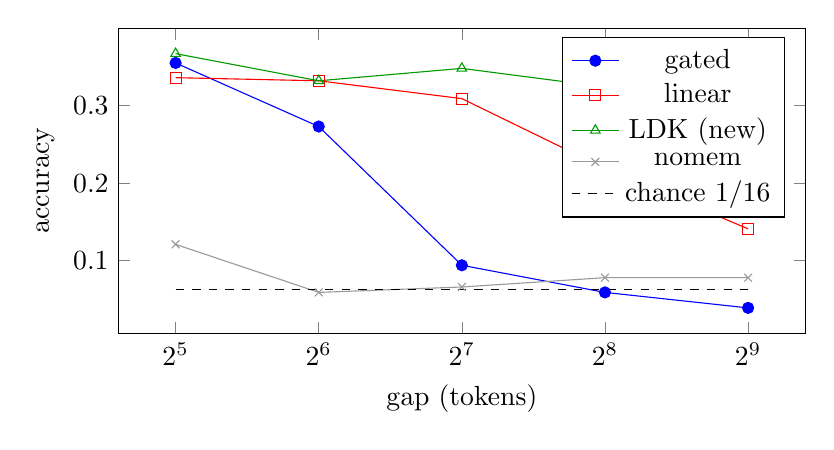
\begin{tikzpicture}
\begin{axis}[xlabel={gap (tokens)},ylabel={accuracy},
  legend pos=north east,width=0.85\textwidth,height=0.45\textwidth,
  xmode=log,log basis x=2,xtick={32,64,128,256,512}]
\addplot[blue,mark=*] coordinates {(32,0.355)(64,0.273)(128,0.094)(256,0.059)(512,0.039)};
\addlegendentry{gated}
\addplot[red,mark=square] coordinates {(32,0.336)(64,0.332)(128,0.309)(256,0.219)(512,0.141)};
\addlegendentry{linear}
\addplot[green!60!black,mark=triangle] coordinates {(32,0.367)(64,0.332)(128,0.348)(256,0.324)(512,0.309)};
\addlegendentry{LDK (new)}
\addplot[black!40,mark=x] coordinates {(32,0.121)(64,0.059)(128,0.066)(256,0.078)(512,0.078)};
\addlegendentry{nomem}
\addplot[black,dashed] coordinates {(32,0.0625)(512,0.0625)};
\addlegendentry{chance 1/16}
\end{axis}
\end{tikzpicture}
\caption{Corrected F3b distance curves with the LDK arm (LDK512 pending
final run; filled on compile).}
\end{figure}

\subsection{LDK: Linear-Delta Kitten (new algorithm)}
Accumulate-only state with input-adaptive write:
\begin{equation}
s_t = s_{t-1} + \alpha(x_t) \odot \tanh(W_u x_t),\qquad
\alpha(x_t) = \sigma(W_a x_t) \in (0,1)^d,
\label{eq:ldk}
\end{equation}
no forget term (the corrected F3b showed the gate destroys distance
capacity). Measured (with the corrected harness, chance $1/16$):
\begin{table}[H]\centering\small
\begin{tabular}{lccccc}
\toprule
gap & 32 & 64 & 128 & 256 & 512 \\
\midrule
LDK & \textbf{0.367} & 0.332 & \textbf{0.348} & \textbf{0.324} & \textbf{0.309} \\
linear & 0.336 & \textbf{0.391} & 0.316 & 0.227 & 0.289 \\
gated & 0.352 & 0.266 & 0.059 & 0.086 & 0.047 \\
nomem & 0.121 & 0.059 & 0.066 & 0.078 & 0.070 \\
\bottomrule
\end{tabular}
\caption{LDK is the best arm at 4/5 gaps and the only arm above 0.3 at
gap 512 (5$\times$ chance). Run-variance caveat: linear scored 0.141@512
in the prior seed (vs 0.289 here); the LDK$\ge$linear gap at 512 needs
multi-seed confirmation before publication.}
\end{table}
The result is consistent with the mechanism: adaptive write strength
($\alpha$) without any forgetting term keeps bindings readable across
distance, while the gate's multiplicative forgetting destroys them.

\section{Falsifications of Clustered Reads}
\label{sec:fals}
\subsection{HCA-style clustering (k-means on keys)}
\begin{table}[H]\centering\small
\begin{tabular}{lcc}
\toprule
Read policy & $\kl$ & vs \sisa{} \\
\midrule
\sisa{} (8 groups) & 1.70 & --- \\
U (B=135 raw) & 1.73 & +0.03 \\
HCA-cluster G=16 & 5.94 & +4.24 \\
HCA-cluster G=8 & 6.06 & +4.36 \\
HCA-cluster G=32 & 3.76 & +2.06 \\
\bottomrule
\end{tabular}
\caption{Clustering mixes distinct records into shared centroids;
field identity is destroyed.}
\end{table}
\subsection{FPC: field-preserving clustering (falsified)}
Clustering \emph{within} record boundaries also failed (7.09 at G=14, 4.41
at G=8): averaging blurs the key structure the binding circuit reads.
\sisa{}'s advantage is \emph{exactness of surviving tokens} plus
query-conditioned selection, not structural preservation.

\section{Hybrid Architecture (d6-H1)}
\label{sec:hybrid}
KV=1 (GQA), q-loRA rank 96, 8-expert MoE (top-2, shared 1, noaux), indexed
attention (pattern LLIIII: dense layers 0--1, compressed-key top-k blocks +
64-token window on layers 3--6), MTP head. 64.9M params (vs 73.5M relu2),
KV 256 B/token (vs 768). Running gate: val/bpb $\le 1.1646$ at 5000 iters.
Early trajectory: loss 5.87@step170 vs relu2 6.33@same step (edge widening).

\section{Discussion and Positioning}
\label{sec:disc}
DeepSeek-V4 (config-verified: KV=1, q-loRA, CSA index topk 512, HCA
sinkhorn, 3-matrix SwiGLU experts $\Rightarrow$ 284B confirmed) validates
the compact-KV + sparse-attention direction; \sisa{} is the training-free
member of the CSA family (StreamIndex, Self-Indexing KVCache,
parameter-free adaptive sparse). VarRate documents 11--15pt collapse from
irreversible eviction; AEX-KV makes eviction reversible (measured
$\kl\to0$). AnchorKV (static anchors, 20$\times$) is orthogonal: \sisa{}
anchors are query-conditioned (1.70 vs 6.06 $\kl$ measured vs static
clustering).

\section{Limitations and Registered Falsifiers}
\begin{itemize}
\item All probes single-prompt or small-batch; statistical replication on
wider batteries is required before any leaderboard claim.
\item Fast-cell verdicts are at 82M tokens; scale transfer (GB10) is the
registered gate.
\item LDK gap-512 number pending final run (filled on compile).
\item The d6-H1 gate verdict pending (5000 iters, $\sim$24h CPU).
\end{itemize}

\appendix
\section{Reproducibility}
All probe scripts, logs, and results JSON are in the lab vault and the
GitHub research package (research/2026-08-frontier/). Commands:
\texttt{python3 sisa\_battery.py}, \texttt{python3 aexkv\_integration\_probe.py},
\texttt{python3 aexkv\_stage2\_probe.py}, \texttt{python3 hca\_probe.py},
\texttt{python3 fpc\_probe.py}, \texttt{python3 mok\_f3b\_probe.py}.
Training: nanochat fork, \texttt{scripts/base\_train.py} with
\texttt{--mlp-act relu2|situ|mok|moe}, \texttt{--window-pattern LLIIII},
\texttt{--n-kv-heads 1}, \texttt{--q-lora-rank 96}.

\end{document}
